\documentclass{article}

% if you need to pass options to natbib, use, e.g.:
%     \PassOptionsToPackage{numbers, compress}{natbib}
% before loading neurips_2025

% The authors should use one of these tracks.
% Before accepting by the NeurIPS conference, select one of the options below.
% 0. "default" for submission
 \usepackage{neurips_2025}
% the "default" option is equal to the "main" option, which is used for the Main Track with double-blind reviewing.
% 1. "main" option is used for the Main Track
%  \usepackage[main]{neurips_2025}
% 2. "position" option is used for the Position Paper Track
%  \usepackage[position]{neurips_2025}
% 3. "dandb" option is used for the Datasets & Benchmarks Track
 % \usepackage[dandb]{neurips_2025}
% 4. "creativeai" option is used for the Creative AI Track
%  \usepackage[creativeai]{neurips_2025}
% 5. "sglblindworkshop" option is used for the Workshop with single-blind reviewing
 % \usepackage[sglblindworkshop]{neurips_2025}
% 6. "dblblindworkshop" option is used for the Workshop with double-blind reviewing
%  \usepackage[dblblindworkshop]{neurips_2025}

% After being accepted, the authors should add "final" behind the track to compile a camera-ready version.
% 1. Main Track
 % \usepackage[main, final]{neurips_2025}
% 2. Position Paper Track
%  \usepackage[position, final]{neurips_2025}
% 3. Datasets & Benchmarks Track
 % \usepackage[dandb, final]{neurips_2025}
% 4. Creative AI Track
%  \usepackage[creativeai, final]{neurips_2025}
% 5. Workshop with single-blind reviewing
%  \usepackage[sglblindworkshop, final]{neurips_2025}
% 6. Workshop with double-blind reviewing
%  \usepackage[dblblindworkshop, final]{neurips_2025}
% Note. For the workshop paper template, both \title{} and \workshoptitle{} are required, with the former indicating the paper title shown in the title and the latter indicating the workshop title displayed in the footnote.
% For workshops (5., 6.), the authors should add the name of the workshop, "\workshoptitle" command is used to set the workshop title.
% \workshoptitle{WORKSHOP TITLE}

% "preprint" option is used for arXiv or other preprint submissions
 % \usepackage[preprint]{neurips_2025}

% to avoid loading the natbib package, add option nonatbib:
%    \usepackage[nonatbib]{neurips_2025}

\usepackage[utf8]{inputenc} % allow utf-8 input
\usepackage[T1]{fontenc}    % use 8-bit T1 fonts
\usepackage{hyperref}       % hyperlinks
\usepackage{url}            % simple URL typesetting
\usepackage{booktabs}       % professional-quality tables
\usepackage{amsmath}
\usepackage{amssymb}
\usepackage{amsfonts}       % blackboard math symbols
\usepackage{nicefrac}       % compact symbols for 1/2, etc.
\usepackage{microtype}      % microtypography
\usepackage{xcolor}         % colors
\usepackage{listings}
\usepackage{graphicx}


% Note. For the workshop paper template, both \title{} and \workshoptitle{} are required, with the former indicating the paper title shown in the title and the latter indicating the workshop title displayed in the footnote. 
\title{Beyond Aggregate Accuracy: Fine-Grained Error Analysis and Prompt Sensitivity in LLM Mathematical Reasoning}


% The \author macro works with any number of authors. There are two commands
% used to separate the names and addresses of multiple authors: \And and \AND.
%
% Using \And between authors leaves it to LaTeX to determine where to break the
% lines. Using \AND forces a line break at that point. So, if LaTeX puts 3 of 4
% authors names on the first line, and the last on the second line, try using
% \AND instead of \And before the third author name.

\hypersetup{
  pdfauthor={},
  pdftitle={},
  pdfsubject={},
  pdfkeywords={},
  pdfcreator={},
  pdfproducer={}
}
\author{Anonymous}

  
  % examples of more authors
  % \And
  % Coauthor \\
  % Affiliation \\
  % Address \\
  % \texttt{email} \\
  % \AND
  % Coauthor \\
  % Affiliation \\
  % Address \\
  % \texttt{email} \\
  % \And
  % Coauthor \\
  % Affiliation \\
  % Address \\
  % \texttt{email} \\
  % \And
  % Coauthor \\
  % Affiliation \\
  % Address \\
  % \texttt{email} \\



\begin{document}


\maketitle 


\begin{abstract}
Large language models (LLMs) exhibit impressive yet unreliable mathematical 
reasoning. Standard evaluations that focus solely on aggregate accuracy mask 
critical error patterns, dataset artifacts, and evaluation noise. In this work, 
we present a fine-grained empirical analysis of LLM errors on GSM8K and the 
Algebra subset of MATH using two Qwen model variants (Qwen-Plus and 
Qwen-Turbo) under multiple prompting strategies. We first conduct a systematic 
error taxonomy on GSM8K, identifying interpretation ambiguity and 
over-reasoning as dominant failure modes and exposing seven dataset-level 
annotation errors that are misattributed to the model. We then design an 
iterative re-evaluation protocol and find that prompt-based error recovery is 
highly unstable: only 4.1\% of initially wrong answers are consistently 
fixed, while over 80\% never recover, revealing substantial stochastic 
variability that undermines single-run evaluations. Furthermore, 
cross-benchmark and cross-model experiments demonstrate that prompting 
efficacy is not universal but jointly determined by model capability and 
task characteristics; strong models achieve near-perfect accuracy with 
prompt saturation, whereas weaker models can suffer from cognitive overload 
with few-shot exemplars on multi-step algebraic tasks. Our findings caution 
against overinterpreting single-run accuracy differences and advocate for 
stability-aware, dataset-audited evaluation protocols in LLM mathematical 
reasoning research.
\end{abstract}

\section{Introduction}

Large Language Models (LLMs) have demonstrated remarkable capabilities across a wide spectrum of tasks, yet mathematical reasoning remains a notable challenge. Compared with natural language understanding tasks, mathematical problem-solving demands precise multi-step logical deduction, accurate numerical computation, and faithful adherence to problem constraints \cite{cobbe2021training, hendrycks2021measuring}. 

Despite significant progress brought by techniques such as Chain-of-Thought (CoT) prompting \cite{wei2022chain} and its zero-shot variant \cite{kojima2022large}, many existing evaluations primarily focus on aggregate accuracy metrics, leaving the underlying error mechanisms insufficiently examined.

A critical yet underexplored question is: \textit{to what extent do model failures reflect genuine reasoning deficiencies versus artifacts of the evaluation process itself?} Recent studies have highlighted that benchmarks such as GSM8K may contain noisy annotations and ambiguous formulations that confound assessment \cite{kismath2024, prolog2024}, including incorrect ground-truth answers and underspecified constraints. Moreover, the sensitivity of LLM outputs to prompt variations and the stochastic nature of generation introduce additional complexity rarely accounted for in single-run evaluations, raising concerns about the reliability of current benchmarking practices.

In this work, we present a comprehensive empirical study that goes beyond aggregate accuracy to investigate the \textit{quality, stability, and fixability} of LLM mathematical reasoning. We evaluate the Qwen model family on two widely-used benchmarks---GSM8K and MATH \cite{hendrycks2021measuring}---under three prompting strategies: Direct prompting, Zero-shot CoT, and Few-shot CoT. Our experimental design incorporates an iterative re-evaluation protocol, where incorrectly answered questions are repeatedly fed back to the model with augmented prompts, enabling a fine-grained analysis of error recovery patterns.

Our experiments yield several key findings. First, a notable portion of GSM8K errors stem from dataset-level issues---semantic ambiguity, underspecified formats, and contradictions between problem statements and reference solutions---that are erroneously penalized as model failures. Second, the stability of error recovery varies markedly across error categories, with some errors being consistently fixed while others exhibit high stochastic variability across repeated trials. Third, prompting efficacy is jointly modulated by model capability and task characteristics: stronger models (Qwen-Plus) achieve near-saturation on MATH-Algebra regardless of prompt choice, while weaker models (Qwen-Turbo) benefit from CoT prompting yet remain vulnerable to formatting errors.

Our main contributions are as follows:
\begin{itemize}
    \item We conduct a systematic error attribution analysis on GSM8K, revealing that a non-negligible proportion of model failures stem from dataset-level issues---including semantic ambiguity, potentially incorrect annotations, and underspecified format requirements---rather than pure reasoning deficiencies.
    
    \item We propose an iterative re-evaluation protocol to assess the fixability and stability of different error categories under targeted prompt augmentation. Our results reveal significant stochastic variability in model recovery, suggesting that single-run evaluations may yield unreliable estimates of model performance.
    
    \item Through comparative experiments across two benchmarks and two model scales, we demonstrate that prompting strategy efficacy is jointly determined by model capability and task characteristics.
\end{itemize}


\section{Related work}

\subsection{Mathematical reasoning in LLMs}
GSM8K \cite{cobbe2021training} and MATH \cite{hendrycks2021measuring} are standard benchmarks for LLM mathematical reasoning, comprising grade-school word problems and competition-level problems across algebra, geometry, and number theory, respectively. More recently, in-context learning strategies have shown that LLMs can achieve competitive performance without parameter updates through carefully designed prompts \cite{brown2020language}.

\subsection{Prompting strategies for reasoning}
Chain-of-Thought (CoT) prompting \cite{wei2022chain} improves LLM mathematical performance by providing exemplars with explicit step-by-step reasoning. Building on this, Kojima et al. \cite{kojima2022large} showed that a simple zero-shot instruction---\textit{Let's think step by step}---can elicit similar reasoning behavior without demonstrations, a technique known as Zero-shot CoT. Wang et al. 

While these methods have been extensively evaluated in terms of overall accuracy, fine-grained analyses of \textit{which} error types are amenable to prompting interventions remain scarce. Our work addresses this gap by systematically categorizing errors and studying their fixability under different prompting conditions.

\subsection{Evaluation challenges and benchmark limitations}
Benchmark annotation errors and format ambiguity have been noted as confounding factors \cite{kismath2024, prolog2024, jo2025finding}. Answer extraction in math benchmarks---parsing free-form outputs into final answers---introduces evaluation noise, particularly in MATH where diverse symbolic representations (e.g., $\frac{1}{2}$ vs.\ $0.5$) cause correct reasoning to be marked incorrect \cite{jo2025finding, hendrycks2021measuring}. Furthermore, the inherent stochasticity of LLM generation means that single-run evaluations may not reliably capture model capabilities \cite{potamitis2025reasonbench, atil2025nondeterminism}. Our work contributes by explicitly modeling format sensitivity and output stability as important evaluation dimensions, rather than treating them as negligible noise.

\section{Methodology}

\subsection{Task formulation}
We formulate mathematical reasoning as a conditional sequence generation task. Given a math problem text $x$, the Large Language Model (LLM) is tasked with generating a response $\hat{y}$ that ideally contains a  reasoning trace followed by a final answer. Let $y^*$ denote the ground-truth answer for $x$. 

The primary evaluation metric is the answer-level accuracy, defined as:
\begin{equation}
    \text{Accuracy} = \frac{1}{N} \sum_{i=1}^{N} \mathbb{I}\big(\text{Match}(\hat{y}_i, y^*_i)\big)
\end{equation}
where $N$ is the total number of evaluated questions, $\mathbb{I}(\cdot)$ is the indicator function, and $\text{Match}(\cdot, \cdot)$ is our custom equivalence judgment function detailed in Section~\ref{sec:extraction}.

\subsection{Answer extraction and evaluation}
\label{sec:extraction}
Accurate answer extraction and matching are essential for math reasoning evaluation, yet they are often overlooked or oversimplified in existing benchmarks. To ensure full reproducibility and minimize evaluation noise, we design separate, strictly rule-based pipelines for GSM8K and MATH without relying on external symbolic solvers  or auxiliary LLMs.

\paragraph{GSM8K.} The official format is \texttt{\#\#\#\# number}. We prompt models to follow this convention. We extract the last numeric token after the final \texttt{\#\#\#\#} marker (or from the full response if absent), strip formatting symbols (\$, commas), and compare with the ground truth via exact numerical equality. Responses without an identifiable answer are treated as incorrect.

\paragraph{MATH.} Answers are LaTeX expressions in \texttt{\textbackslash boxed\{\}}. Our pipeline comprises three stages: (1) \textit{localization}---extract the last \texttt{\textbackslash boxed\{\}} via brace-counting, falling back to explicit markers, last-line, or numeric extraction; (2) \textit{normalization}---remove LaTeX formatting commands, unify fraction notations, and strip variable prefixes; (3) \textit{equivalence judgment}---a cascade of exact match, normalized match, float comparison ($10^{-6}$ tolerance), and fraction-aware comparison. Full regex specifications and the complete cascade are provided in Appendix~\ref{app:pipeline}.
\textit{(There are very few format blind spots in the automatic extraction, which will be supplemented by manual review in Section~\ref{sec:experiments}.)}

\subsection{Prompt strategies}
\label{sec:prompts}
Inspired by prior work on Chain-of-Thought (CoT) reasoning~\cite{wei2022chain, kojima2022large}, we evaluate three prompting strategies on the first 300 questions of the GSM8K and MATH test sets to isolate the impact of reasoning elicitation. All prompts are appended as instructions to the end of the original problem text. (Full prompt templates are provided in Appendix~\ref{app:prompts}).

\begin{itemize}
    \item \textbf{Zero-shot CoT:} Guides the model to reason step-by-step without providing examples. For GSM8K, it explicitly requests the \texttt{\#\#\#\#} format, forbids thousand separators, and includes a reminder for unit conversions. For MATH, it mandates the use of \texttt{\textbackslash boxed\{\}} and LaTeX formatting.
    \item \textbf{Direct Prompting (No CoT):} Removes the step-by-step reasoning instruction, directly requesting the final answer in the specified format. This serves as our baseline to measure the pure gain from CoT.
    \item \textbf{Few-shot CoT:} Replaces the verbal reasoning instruction with 5 in-context examples drawn from outside the 300-question evaluation set to prevent data leakage. 
    \begin{itemize}
        \item \textit{For GSM8K:} To ensure diverse coverage, we manually categorize the problem types and select one error-free exemplar with its official solution for each category.
        \item \textit{For MATH:} Since the first 300 questions are exclusively algebra problems, we randomly sample 5 algebra problems with official solutions as exemplars.
    \end{itemize}
    Each exemplar consists of a problem statement and a complete standard reasoning process, preceded by an instruction to learn from the examples.
\end{itemize}

\subsection{Iterative re-evaluation protocol}
\label{sec:reeval}
To systematically investigate the fixability of specific error types and the output stability of mathematical reasoning, we design an iterative re-evaluation protocol, applied specifically to the GSM8K dataset. 

The protocol initializes with the Zero-shot CoT prompt (excluding the unit conversion reminder) and conducts multiple evaluation rounds on the same problem set. Let $\mathcal{E}_t$ denote the set of incorrectly answered questions at round $t$.

\textbf{Procedure:}
\begin{enumerate}
    \item \textit{Initial Evaluation ($t=0$):} Run the model on all problems using the base Zero-shot CoT prompt. Determine correctness via Section~\ref{sec:extraction} to obtain the initial error set $\mathcal{E}_0$.
    \item \textit{Prompt Refinement:} For each problem in $\mathcal{E}_t$, keep the problem text unchanged but append a targeted reminder to the prompt: \textit{``and pay attention to unit conversions.''} The model weights  remain strictly identical.
    \item \textit{Re-evaluation:} Re-run the model exclusively on the problems in $\mathcal{E}_t$ using the refined prompt, extract new answers, and re-judge correctness to obtain $\mathcal{E}_{t+1}$.
    \item \textit{Iteration:} Repeat steps 2--3 for $T$ additional rounds. In this work, we set $T=3$, resulting in a total of 4 runs (1 initial + 3 re-evaluations).
\end{enumerate}

\textbf{Reporting convention:}
The objective of this protocol is to observe performance fluctuations as the prompt is incrementally strengthened. Therefore, we report the accuracy and error composition of each round independently. This experimental design allows us to cleanly disentangle two distinct phenomena: the intrinsic stochastic variability of the LLM (observable when the same prompt yields different results across runs) and the systematic performance gain derived from targeted prompt reinforcement.


\section{Experiments and results}
\label{sec:experiments}
\subsection{Implementation details}
All experiments are conducted via the official Qwen API using the \texttt{Generation.call} interface. We evaluate two model scales: Qwen-Plus and Qwen-Turbo. Unless otherwise specified, we adopt the API's default decoding configuration to assess the models' out-of-the-box capabilities: temperature $= 0.7$, top-$p = 0.8$. 
\subsection{RQ1: error categorization and fixability on GSM8K}
\label{sec:rq1}
\subsubsection{Baseline performance}
We first establish the baseline performance of Qwen-Plus on the full GSM8K test set (1{,}319 questions) using the Zero-shot CoT prompt (excluding the unit-conversion reminder). The model achieves an accuracy of $96.29\%$ ($49$ errors), providing a solid foundation for subsequent fine-grained error analysis.
\subsubsection{Error distribution and dataset-level issues}
\label{sec:dataset_errors}

We manually categorize the 49 incorrect predictions into six error types. As Figure~\ref{fig:pie_chart1} in Appendix~\ref{app:main} illustrates, \textit{Interpretation Ambiguity} and \textit{Over-reasoning} constitute the largest proportions, indicating that the model's errors primarily stem from misinterpretation of problem statements rather than computational deficiencies. To some extent, this also reflects inherent semantic ambiguity within certain questions in the dataset itself.
More critically, during manual inspection we identify \textbf{7 problems} (IDs: 256, 455, 824, 953, 1039, 1043, 1310) for which the ground-truth solution is fundamentally inconsistent with the problem statement. 
We independently recomputed all 7 problems and confirmed that the model's outputs are mathematically correct. These cases are reclassified into a distinct \textit{Dataset Annotation Error} category (see Figure~\ref{fig:annotation_errors} in Appendix~\ref{app:dataset_errors} for all the cases). This finding corroborates recent observations on GSM8K annotation quality and underscores that a non-trivial fraction of reported ``model errors'' are in fact evaluation artifacts.

\subsubsection{Iterative re-evaluation: non-monotonic gains}
\label{sec:iterative}

To investigate whether targeted prompt augmentation can repair specific error types, and whether such repairs are stable, we apply the Iterative Re-evaluation Protocol described in Section~\ref{sec:reeval}. Specifically:
\begin{enumerate}
    \item \textbf{RF1 (Control re-run):} The 49 incorrectly answered questions are re-fed to the model with the \textit{identical} Zero-shot CoT prompt (no modification). This establishes the stochastic baseline for error recovery.
    \item \textbf{RF2--RF4 (Prompt augmentation):} A unit-conversion reminder (``\textit{and pay attention to unit conversions}'') is appended to the prompt. The model is re-evaluated on the same 49 questions for three consecutive runs.
\end{enumerate}
\begin{figure}[t]
    \centering
    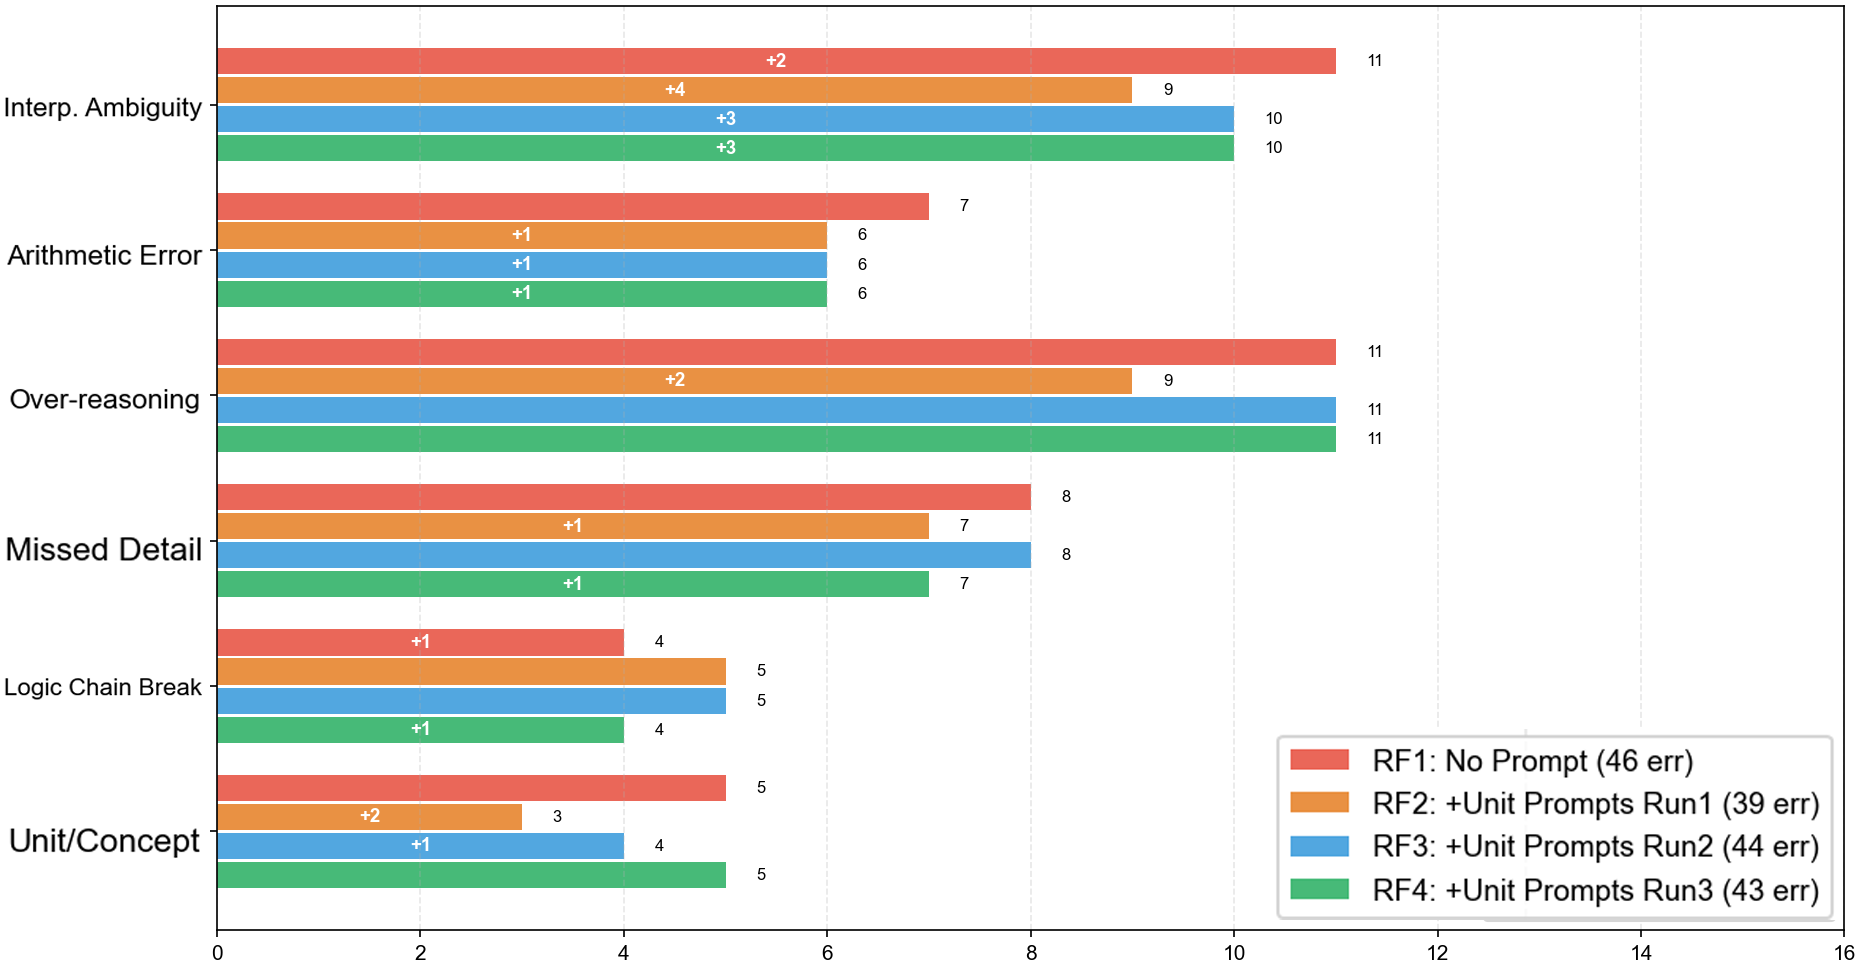
\includegraphics[width=\columnwidth]{figures/bar_comparison.png}
    \caption{Per-category error counts across four evaluation rounds on the 49 incorrectly answered GSM8K problems. RF1 re-runs the original prompt; RF2--RF4 append a unit-conversion reminder. The non-monotonic trajectory (46$\to$39$\to$44$\to$43) indicates that prompt augmentation yields inconsistent, run-dependent gains.}
    \label{fig:bar_comparison}
\end{figure}

As shown in Figure~\ref{fig:bar_comparison}, the control re-run (RF1) reduces errors from 49 to 46, confirming the presence of stochastic variability even without prompt modification. Appending the unit-conversion reminder (RF2--RF4) further reduces errors to 39--44, but the improvement is \textbf{non-monotonic and run-dependent}: RF2 achieves the best result (39 errors), yet RF3 regresses to 44 before partially recovering in RF4 (43). At the category level, the \textit{Unit/Concept} errors show the largest relative reduction (from 5 to 3--4), suggesting that explicit reminders can marginally mitigate format-related confusion. However, categories such as \textit{Interpretation Ambiguity} and \textit{Over-reasoning} remain largely invariant, indicating that these errors are structurally entrenched and insensitive to surface-level prompt augmentation.

\subsubsection{Recovery stability: the rarity of consistent fixes}
\label{sec:stability}

We further analyze the \textit{stability} of error recovery across the three prompt-augmented runs (RF2--RF4). See Figure~\ref{fig:fix_stability_by_cat1} in Appendix~\ref{app:main} for details.

The high degree of stochastic variability carries an important methodological implication: \textbf{observing a ``fix'' in a single re-run may be a spurious signal rather than evidence of genuine capability improvement}. Our results underscore the necessity of multi-run stability analysis in error attribution studies and validate the design choice in Section~\ref{sec:reeval} to report each round independently rather than aggregating via union or intersection.

\subsection{RQ2: cross-model, cross-task prompting analysis}
\label{sec:rq2}

\subsubsection{GSM8K (Q1--300): Marginal Prompt Sensitivity}
\label{sec:gsm300}

We compare three prompting strategies (Zero-shot CoT, Direct Prompting, Few-shot CoT) on a controlled subset of the first 300 questions of the GSM8K test set, using Qwen-Plus.

As shown in Figure~\ref{fig:gsm300_accuracy1} in Appendix~\ref{app:main}, Zero-shot CoT and Few-shot CoT achieve \textit{identical} accuracy (95.7\%, 13 errors each), while Direct Prompting (No-CoT) trails marginally at 95.0\% (15 errors). The negligible inter-strategy gap indicates that, for a capable model on a relatively simple benchmark, prompt engineering yields diminishing returns---a phenomenon we term \textit{prompt saturation}.
Crucially, \textbf{6 questions are incorrectly answered by all three strategies} (see Figure~\ref{fig:gsm300_comparison} in Appendix~\ref{app:gsm300_errors} for the detailed comparison). Manual inspection reveals that this shared failure set includes Q256, a confirmed dataset-level annotation error (Section~\ref{sec:dataset_errors}), along with several problems exhibiting severe semantic ambiguity. The fact that even the strongest prompting configuration cannot resolve these cases suggests that their failures are \textit{fundamentally irrecoverable via prompt engineering}.
An additional observation merits attention: although Few-shot CoT and Zero-shot CoT achieve identical overall accuracy, their \textit{error distributions differ}---Few-shot fixes 6 questions that Zero-shot misses, while regressing on 6 others. (see Figure~\ref{fig:gsm300_comparison} in Appendix~\ref{app:gsm300_errors})This \textbf{zero-sum redistribution} indicates that in-context exemplars primarily shift the model's reasoning style rather than uniformly improving reasoning quality.

\subsubsection{MATH-Algebra (Q1--300): capability-dependent ceiling effects}
\label{sec:math300}
We apply the same three prompting strategies to the first 300 questions of the MATH test set (all belonging to the Algebra category), evaluating both Qwen-Plus and Qwen-Turbo to examine how model capability modulates prompt effectiveness.
\paragraph{(a) Qwen-Plus: Near-Perfect Saturation.}

As illustrated in Figure~\ref{fig:plus_math1}in Appendix~\ref{app:main}, Qwen-Plus achieves a raw accuracy of 98\% on MATH-Algebra, with virtually no difference across the three prompting strategies. The flat accuracy curve(bottom-right panel) indicates that the model's intrinsic algebraic reasoning capacity \textit{saturates} this subset---a clear ceiling effect.
Moreover, all 6 errors across all runs are attributable to \textbf{format mismatches} rather than reasoning failures(e.g.predicted \texttt{7(x-3)(x+3)} vs.\ gold \texttt{7(x+3)(x-3)}). 
While Few-shot CoT does not improve accuracy, it marginally increases the exact-match count (from 258 under Zero-shot to 260 under Few-shot), suggesting that in-context exemplars help the model internalize the benchmark's preferred formatting conventions.
\paragraph{(b) Qwen-Turbo: Non-Monotonic Prompt Effects.}
\begin{figure*}[t]
    \centering
    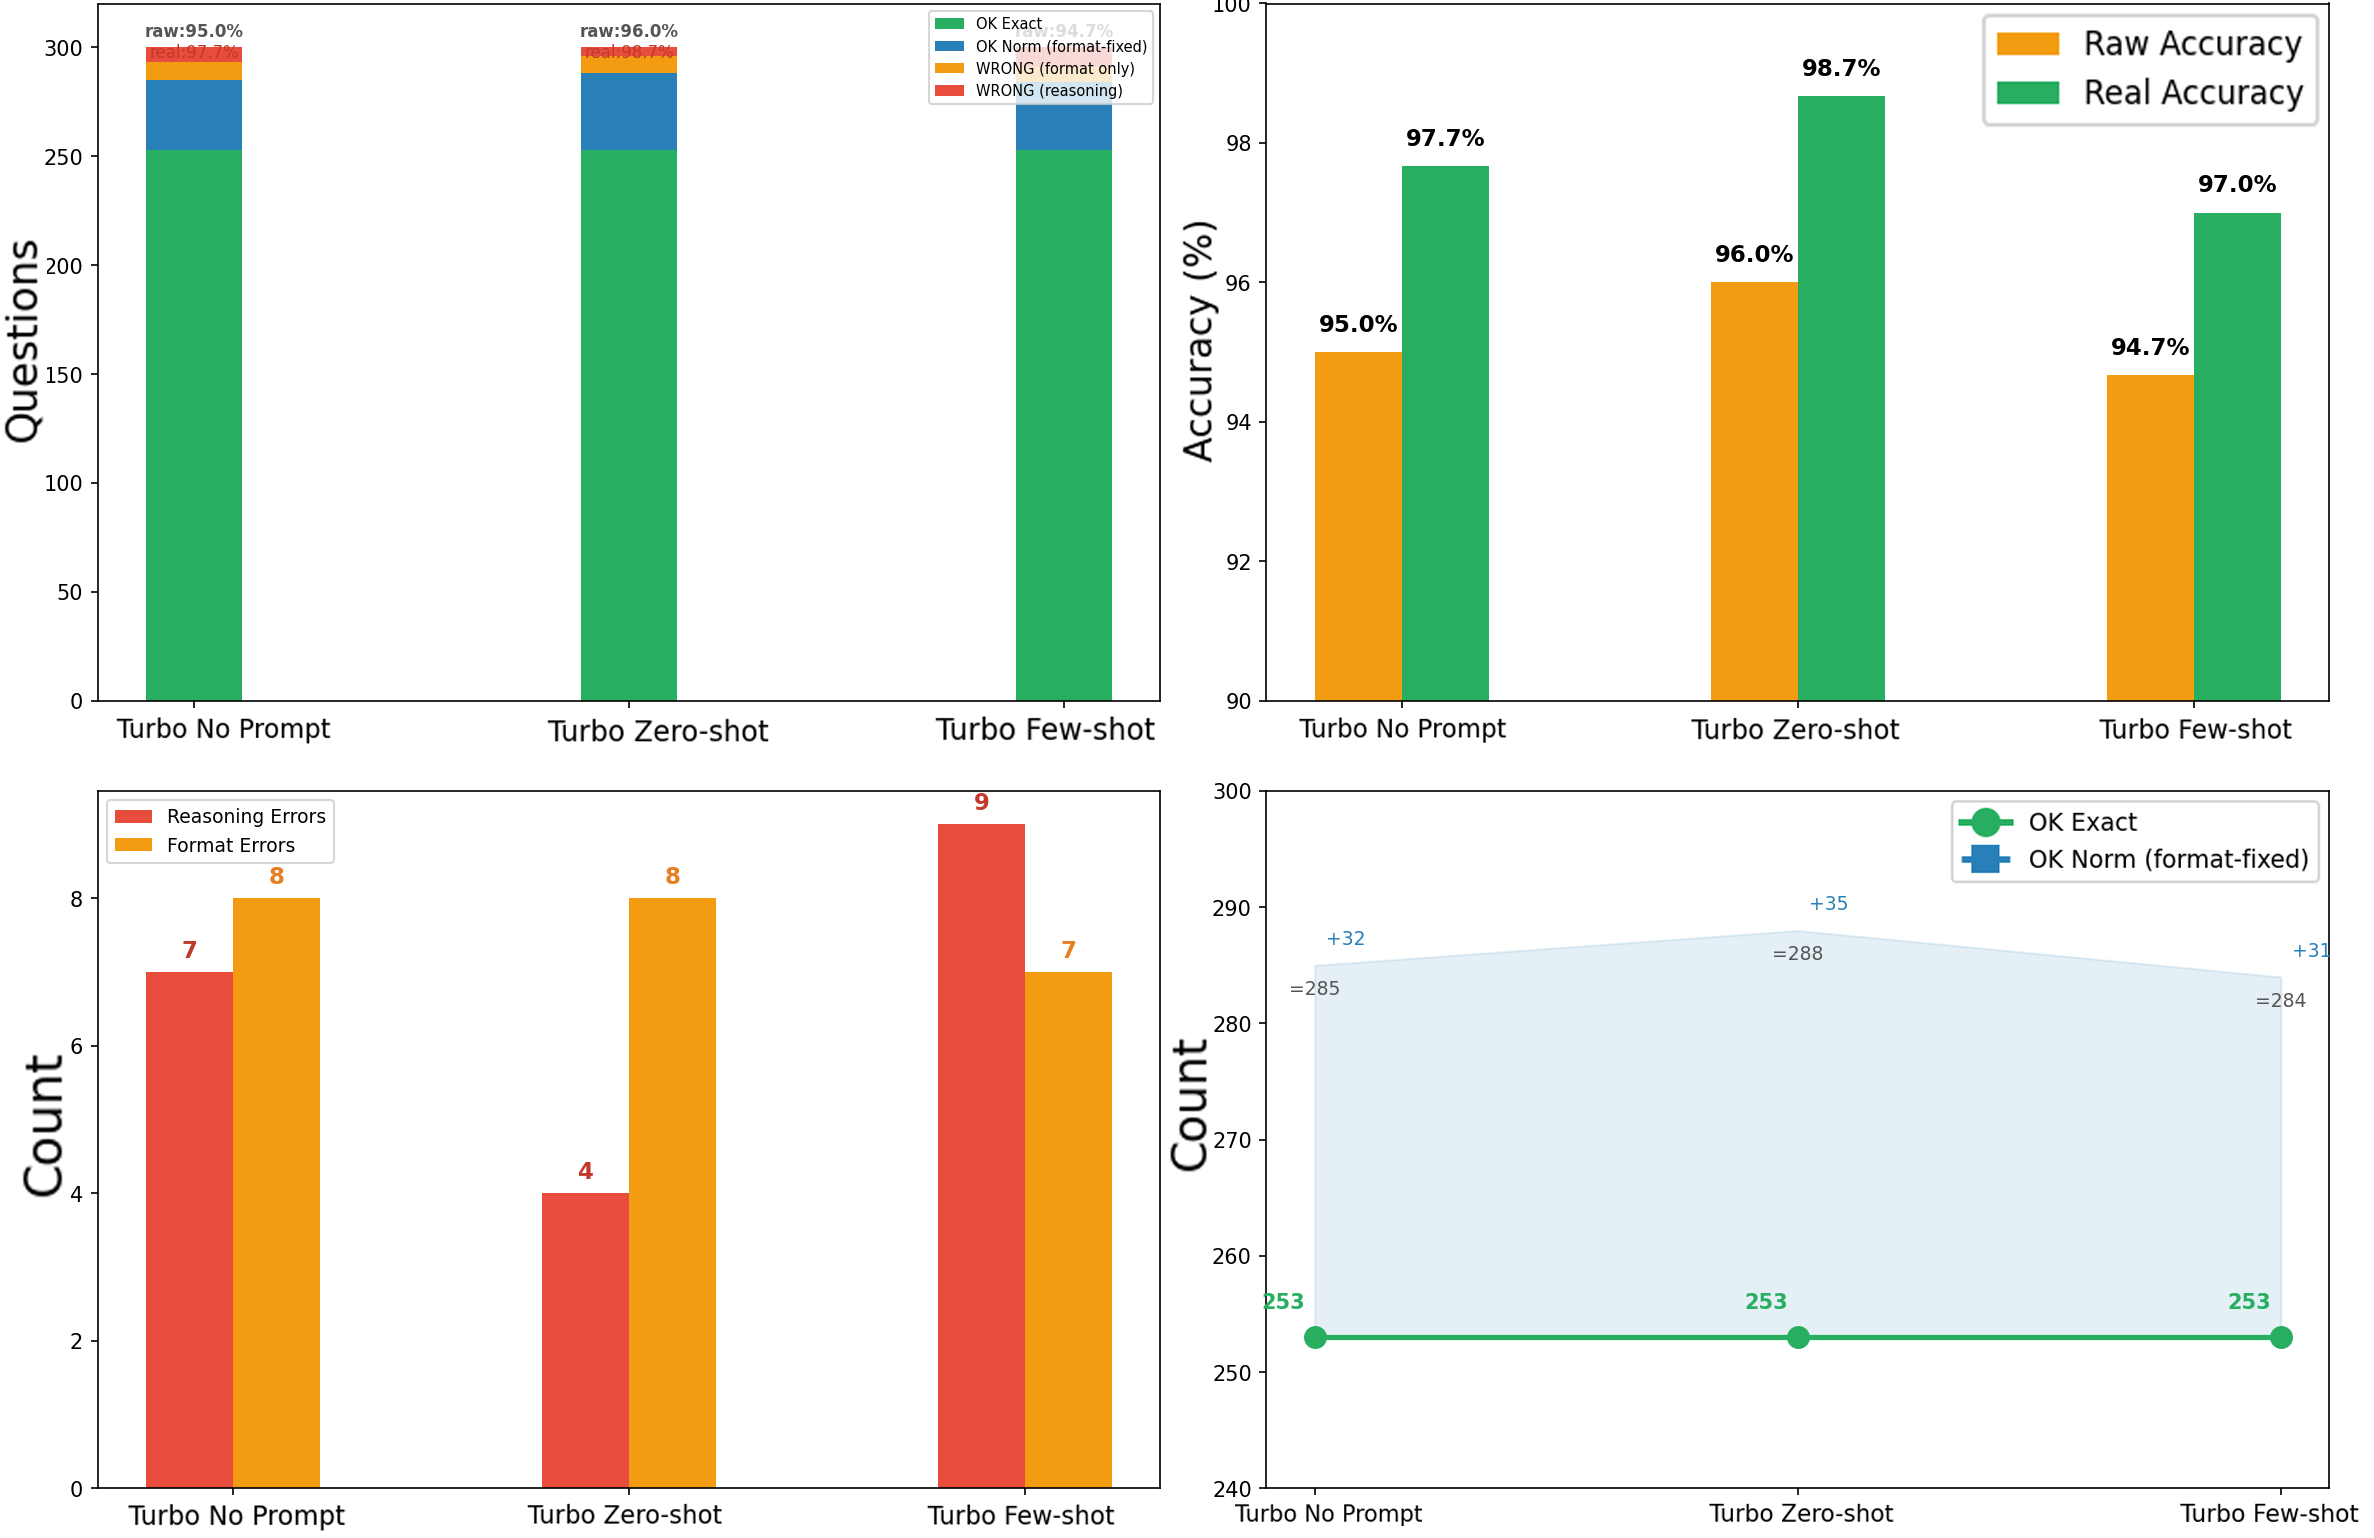
\includegraphics[width=\textwidth]{figures/turbo_comparison_chart.png}
    \caption{MATH-Algebra (Q1--300) evaluation results for Qwen-Turbo. \textbf{Top-left:} Answer matching distribution by strategy. \textbf{Top-right:} Raw vs.\ real accuracy---normalization recovers 2--4\% of format-induced false negatives, revealing the true capability hierarchy (Zero-shot $>$ No-CoT $>$ Few-shot). \textbf{Bottom-left:} Format vs.\ reasoning error decomposition---Few-shot incurs 9 reasoning errors vs.\ only 4 under Zero-shot CoT, despite comparable format error counts. \textbf{Bottom-right:} Exact vs.\ normalized match counts per strategy. The non-monotonic ranking across strategies reveals cognitive overload effects in weaker models.}
    \label{fig:turbo_math}
\end{figure*}
Qwen-Turbo exhibits a \textbf{counterintuitive} performance ranking: Zero-shot CoT (96.0\%) $>$ Direct Prompting (95.0\%) $>$ Few-shot CoT (94.7\%) in terms of raw accuracy. 
The top panel of Figure~\ref{fig:turbo_math} highlights a critical distinction between raw and real accuracy.. After our manual inspection, we eliminate the format mismatches and got the actual accuracy of the model: Zero-shot CoT (98.7\%) $>$ Direct Prompting (97.7\%) $>$ Few-shot CoT (97.0\%). The 2--4\% gap between raw and real accuracy quantifies the prevalence of format-induced false negatives and validates our evaluation design.
Surprisingly, Few-shot CoT \textit{underperforms}on Qwen-Turbo. We attribute this to \textbf{cognitive overload}: the 5 in-context algebra exemplars consume the model's limited context capacity, leaving fewer computational resources for the target problem's symbolic manipulation. The bottom-left panel of Figure~\ref{fig:turbo_math} supports this hypothesis: Few-shot incurs 9 reasoning errors compared to only 4 under Zero-shot CoT, despite having comparable format error counts.
Figure~\ref{fig:turbo_persistent} in Appendix~\ref{app:turbo_errors} lists the reasoning errors that persist across prompting strategies. 

At first glance, our results appear contradictory: on GSM8K, Few-shot CoT matches Zero-shot CoT; on MATH-Algebra, it underperforms. These observations can be \textbf{unified by a single principle}: \textit{prompting efficacy is jointly determined by model capability and task characteristics}.
The non-monotonicity challenges the common assumption that ``more prompting always helps'' and suggests that \textbf{prompt engineering must be calibrated to the specific model--task pair} rather than applied uniformly.
\section{Conclusion}
\label{sec:conclusion}
In this work, we presented a fine-grained empirical study of error behavior and prompt sensitivity in LLMs on mathematical reasoning benchmarks. 
Our three main contributions are: 
(i) a taxonomy revealing interpretation ambiguity and over-reasoning as dominant failure modes, plus 7 dataset-level annotation errors in GSM8K misattributed to models; 
(ii) an iterative re-evaluation protocol showing that prompt-based fixes are highly unstable---only 4.1\% of errors are consistently recovered, while 81.6\% never recover; 
(iii) a non-monotonic interaction between model capability and prompt complexity, where Few-shot CoT underperforms for weaker models on structured tasks due to cognitive overload.
These findings suggest that prompting efficacy must be calibrated to the model--task pair rather than applied uniformly, and that multi-run stability analysis should be a methodological prerequisite in error attribution studies. 
We acknowledge limitations in scope (two model scales, two datasets), reliance on a proprietary API, and the correlational nature of our cognitive overload hypothesis. 
Future work includes extending this framework to open-weight models and developing automated benchmark auditing tools.




%\begin{ack}
%Use unnumbered first level headings for the acknowledgments. All acknowledgments
%go at the end of the paper before the list of references. Moreover, you are required to declare
%funding (financial activities supporting the submitted work) and competing interests (related financial activities outside the submitted work).
%More information about this disclosure can be found at: \url{https://neurips.cc/Conferences/2025/PaperInformation/FundingDisclosure}.
%
%
%Do {\bf not} include this section in the anonymized submission, only in the final paper. You can use the \texttt{ack} environment provided in the style file to automatically hide this section in the anonymized submission.
%\end{ack}


\bibliographystyle{plainnat}
\bibliography{myrefs}


\appendix
\section{Prompt Templates}
\label{app:prompts}

In this section, we provide the exact prompt templates used in our experiments. For the GSM8K dataset, the original prompts used in our experiments were in Chinese to align with the model's primary instruction-tuning language; however, we provide their English translations here for clarity and reproducibility. For the MATH dataset, all prompts were in English.

\subsection{GSM8K Prompts}

\subsubsection{Zero-shot CoT Prompt}
The following instruction is appended to the end of the original problem text:
\begin{quote}
\small
\texttt{\textbackslash n\textbackslash nPlease reason step by step, and write the final answer on a separate line at the end, formatted as '\#\#\#\# answer\_number'. Note that the answer number should be a pure number without separators such as 8,000, and pay attention to unit conversions.}
\end{quote}
\textit{Note: In the initial round of the Iterative Re-evaluation Protocol (Section~\ref{sec:reeval}), the clause ``and pay attention to unit conversions'' is omitted.}

\subsubsection{Direct Prompting (No CoT)}
The reasoning instruction is removed, and the following is appended instead:
\begin{quote}
\small
\texttt{\textbackslash n\textbackslash nPlease write the final answer on a separate line at the end, formatted as '\#\#\#\# answer\_number'. Note that the answer number should be a pure number without separators such as 8,000, and pay attention to unit conversions.}
\end{quote}

\subsubsection{Few-shot CoT Prompt ($k=5$)}
The verbal reasoning instruction is replaced with the following example-learning instruction and 5 exemplars:
\begin{quote}
\small
\texttt{Please read the following example questions and learn the reasoning process of the standard answers.}
\end{quote}

\noindent\textbf{Exemplar 1:}
\begin{quote}
\small
\textbf{Question:} Jen decides to travel to 3 different countries. He has to pay \$400 for the supplies he needs, in total. The tickets for travel cost, in total, 50\% more than the supplies. How much does travel cost? \\
\textbf{Solution:} He pays 400*.5=\$200 more for tickets than supplies. That means the tickets cost 400+200=\$600. So it cost 600+400=\$1000 in total. \#\#\#\# 1000
\end{quote}

\noindent\textbf{Exemplar 2:}
\begin{quote}
\small
\textbf{Question:} Sasha and Julie are best friends playing on opposing basketball teams. The teams have two practice games scheduled. In the first game, Sasha had the home court advantage and scored 14 points. Julie scored 4 fewer points than Sasha in the same game. Sasha always struggles during away games and their second match was at Julie's home court. Sasha scored 6 fewer points in the second game than Julie's score in the first game. How many total points did Sasha score during both games? \\
\textbf{Solution:} In the first game, Sasha scored 14 points, and Julie scored four fewer points: 14-4 = 10 points. In the second game, Sasha scored 6 points fewer than Julie's score in the first game, meaning she scored 10-6=4 points. Sasha scored 10+4=14 points in the two games. \#\#\#\# 14
\end{quote}

\noindent\textbf{Exemplar 3:}
\begin{quote}
\small
\textbf{Question:} Teddy finished half of a 500 piece puzzle, and then started and finished another 500 piece puzzle within an hour. How many puzzle pieces did Teddy place during that hour? \\
\textbf{Solution:} Teddy did 1/2 * 500 pieces = 250 pieces. Teddy completed 250 pieces + 500 pieces = 750 pieces. \#\#\#\# 750
\end{quote}

\noindent\textbf{Exemplar 4:}
\begin{quote}
\small
\textbf{Question:} Chase and Rider can ride their bikes thrice a day for 5 days; but on two other days, they ride twice the times they do on usual days. How many times do they ride their bikes a week? \\
\textbf{Solution:} Each person rides his bike 3 x 5 = 15 times for 5 days. Together, they ride 15+15 = 30 times for five days. Each person rides his bike 3 x 2 = 6 times for every day of the other two days. This means each person rides 6*2 = 12 times on each day of the other two days. The total for the other two days is 12+12 = 24. For the whole week the together ride 24+30 = 54 times. \#\#\#\# 54
\end{quote}

\noindent\textbf{Exemplar 5:}
\begin{quote}
\small
\textbf{Question:} Imma has 3 cats. She feeds her cats twice a day with 60 grams of cat food. How many days will 720 grams of cat food last? \\
\textbf{Solution:} The 3 cats consume 60 grams/cat x 3 cats = 180 grams of food per meal. Since they eat twice a day, then they consume 180 grams/meal x 2 meals/day = 360 grams in a day. So, 720 grams of cat food only last for 720 grams / 360 grams/day = 2 days. \#\#\#\# 2
\end{quote}


\subsection{MATH Prompts}

\subsubsection{Zero-shot CoT Prompt}
The following instruction is appended to the end of the original problem text:
\begin{quote}
\small
\texttt{\textbackslash n\textbackslash nPlease reason step by step, put your final answer inside \textbackslash boxed\{\}. Use LaTeX for mathematical expressions.}
\end{quote}

\subsubsection{Direct Prompting (No CoT)}
The reasoning instruction is removed:
\begin{quote}
\small
\texttt{\textbackslash n\textbackslash nPlease put your final answer inside \textbackslash boxed\{\}. Use LaTeX for mathematical expressions.}
\end{quote}

\subsubsection{Few-shot CoT Prompt ($k=5$)}
The verbal instruction is replaced with the following instruction and 5 randomly sampled algebra exemplars:
\begin{quote}
\small
\texttt{Please study the reasoning process of the solutions in the following example questions.}
\end{quote}

\noindent\textbf{Exemplar 1:}
\begin{quote}
\small
\textbf{Problem:} Evaluate $\left\lceil3\left(6-\frac12\right)\right\rceil$. \\
\textbf{Solution:} Firstly, $3\left(6-\frac12\right)=18-1-\frac12=17-\frac12$. Because $0\le\frac12<1$, we have $\left\lceil17-\frac12\right\rceil=\boxed{17}$.
\end{quote}

\noindent\textbf{Exemplar 2:}
\begin{quote}
\small
\textbf{Problem:} Sam is hired for a 20-day period. On days that he works, he earns \$60. For each day that he does not work, \$30 is subtracted from his earnings. At the end of the 20-day period, he received \$660. How many days did he not work? \\
\textbf{Solution:} Call $x$ the number of days Sam works and $y$ the number of days he does not. We can set up the following system of equations: $x+y = 20$ and $60x - 30y = 660$. Solving for $x$ in the first equation yields $x = 20 - y$. Substituting into the second equation gives $60(20-y) - 30y = 660$. Simplifying yields $-9y = -54$, or $y = 6$. Thus, Sam did not work for $\boxed{6}$ days.
\end{quote}

\noindent\textbf{Exemplar 3:}
\begin{quote}
\small
\textbf{Problem:} Find the center of the circle with equation $x^2 - 6x + y^2 + 2y = 9$. \\
\textbf{Solution:} Completing the square, we get $(x - 3)^2 + (y + 1)^2 = 19$. Therefore, the center of the circle is $\boxed{(3, -1)}$.
\end{quote}

\noindent\textbf{Exemplar 4:}
\begin{quote}
\small
\textbf{Problem:} If $x = 2$ and $y = 5$, then what is the value of $\frac{x^4+2y^2}{6}$? \\
\textbf{Solution:} We have $\frac{x^4 + 2y^2}{6} = \frac{2^4 + 2(5^2)}{6} = \frac{16+2(25)}{6} = \frac{16+50}{6} = \frac{66}{6} = \boxed{11}$.
\end{quote}

\noindent\textbf{Exemplar 5:}
\begin{quote}
\small
\textbf{Problem:} The sequence of integers in the row of squares and in each of the two columns of squares form three distinct arithmetic sequences. What is the value of $N$? (Accompanied by an Asymptote diagram). \\
\textbf{Solution:} Since $18 - 14 = 4$, the common difference in the first column is 4, so the number above 14 is 10, and above 10 is 6. This is the fourth number in the row, so the common difference in the row is $(6 - 21)/3 = -5$. The seventh number in the row is $21 - 5 \cdot 6 = -9$. In the second column, the common difference is $[(-17) - (-9)]/4 = -2$, so $N = -9 - (-2) = \boxed{-7}$.
\end{quote}

\section{Answer Extraction Details}
\label{app:pipeline}

\subsection{GSM8K Extraction}

The official GSM8K answer format is \texttt{\#\#\#\# number}. We prompt models to follow this convention. \textbf{Answer localization} proceeds in two stages: if the generated text contains \texttt{\#\#\#\#}, we extract the substring after its last occurrence and strip \$ signs and commas; otherwise, the same cleaning is applied to the entire response. All numeric tokens matching the regular expression \texttt{[-+]?\textbackslash d*\textbackslash.?\textbackslash d+} are extracted, and the \textit{last} valid token is selected as the final prediction, converted to an integer or float. If no number is found, the prediction is marked as missing.
\textbf{Normalization} solely removes commas and \$ signs. \textbf{Equivalence judgment} relies on exact numerical equality ($\hat{y} == y^*$). Since GSM8K ground truths are strictly integers or finite decimals, this comparison is unambiguous.

\subsection{MATH Extraction}
Answers in the MATH dataset are typically LaTeX expressions enclosed in \texttt{\textbackslash boxed\{\}}. Our pipeline employs a four-layer localization strategy and a cascaded equivalence check.

\textbf{Answer localization} follows a strict priority order:
\begin{enumerate}
    \item \textit{Boxed extraction}: Using brace-counting to handle nested structures, we extract the content of the \textit{last} \texttt{\textbackslash boxed\{...\}} in the text.
    \item \textit{Explicit marker matching}: If Step 1 fails, we search for trigger phrases (e.g., ``the answer is'', ``final answer'') and capture the subsequent substring.
    \item \textit{Last-line extraction}: The last non-empty line, provided it is shorter than 200 characters, is taken as the candidate.
    \item \textit{Numeric fallback}: As a last resort, all LaTeX commands and punctuation are stripped, and the last numeric token is extracted.
\end{enumerate}

The extracted raw string undergoes \textbf{normalization} using purely regex and string operations. Key steps include: stripping \$ wrappers; removing formatting commands (e.g., \texttt{\textbackslash text}, \texttt{\textbackslash mathrm}) and their contents; unifying \texttt{\textbackslash dfrac} to \texttt{\textbackslash frac}; removing \texttt{\textbackslash left}, \texttt{\textbackslash right}, and spacing commands; expanding shorthands (e.g., \texttt{\textbackslash frac12} to \texttt{\textbackslash frac\{1\}\{2\}}); and stripping variable prefixes (e.g., $x=$) and trailing punctuation. Irrational numbers, square roots, and $\pi$ are preserved in symbolic form without numerical approximation.

\textbf{Equivalence judgment} utilizes a cascade of five strategies, returning \texttt{True} upon the first successful match:
\begin{enumerate}
    \item Exact string match of raw answers;
    \item Exact string match post-normalization;
    \item Float comparison with an absolute tolerance of $10^{-6}$ (skipped if safe float conversion fails);
    \item Fraction-aware comparison: parses both \texttt{\textbackslash frac\{a\}\{b\}} and \texttt{a/b}, converts to float, and applies the $10^{-6}$ tolerance;
    \item Exact match after removing all whitespace.
\end{enumerate}

\textbf{Handling Missing and Multiple Answers:} If the pipeline yields a null answer, the response is scored as incorrect. When multiple \texttt{\textbackslash boxed\{\}} instances appear or the model self-corrects during reasoning, the \textit{last} identified answer is always used, assuming the model's final conclusion appears at the end. Potential biases from this assumption are discussed in our error analysis (Section~\ref{sec:experiments}).

%----------------------------------------------------------------------
\section{Experiments' charts}
\label{app:main}
Figure~\ref{fig:pie_chart1} presents the error distributions in the baseline. See Section~\ref{sec:stability}.
\begin{figure}[t]
    \centering
    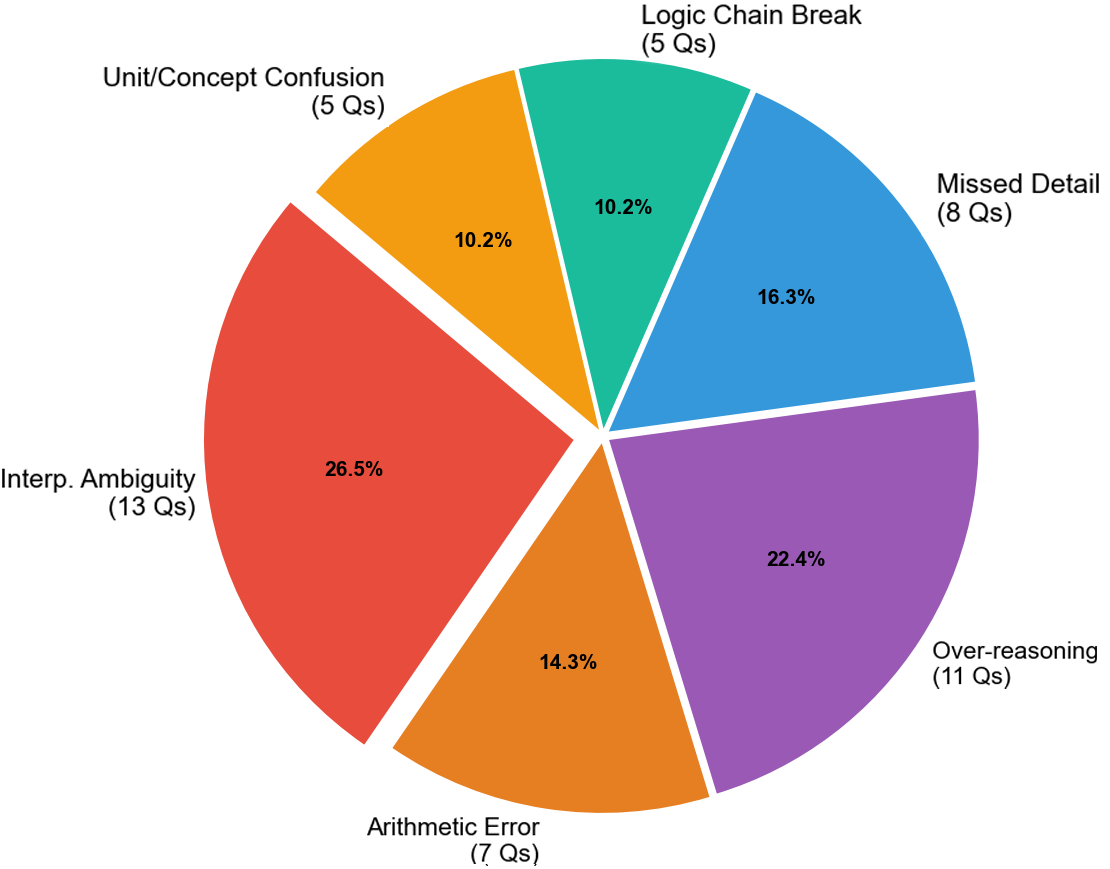
\includegraphics[width=0.75\linewidth]{figures/pie_chart.png}
    \caption{Distribution of error categories across 49 incorrect predictions of Qwen-Plus on the full GSM8K test set under Zero-shot CoT prompting. Interpretation Ambiguity and Over-reasoning dominate, suggesting that dataset-level semantic issues play a non-trivial role.}
    \label{fig:pie_chart1}
\end{figure}

Figure~\ref{fig:fix_stability_by_cat1} provides the Intuitive stability analysis of the fixed problems. See Section~\ref{sec:rq1}.
\begin{figure}[t]
    \centering
    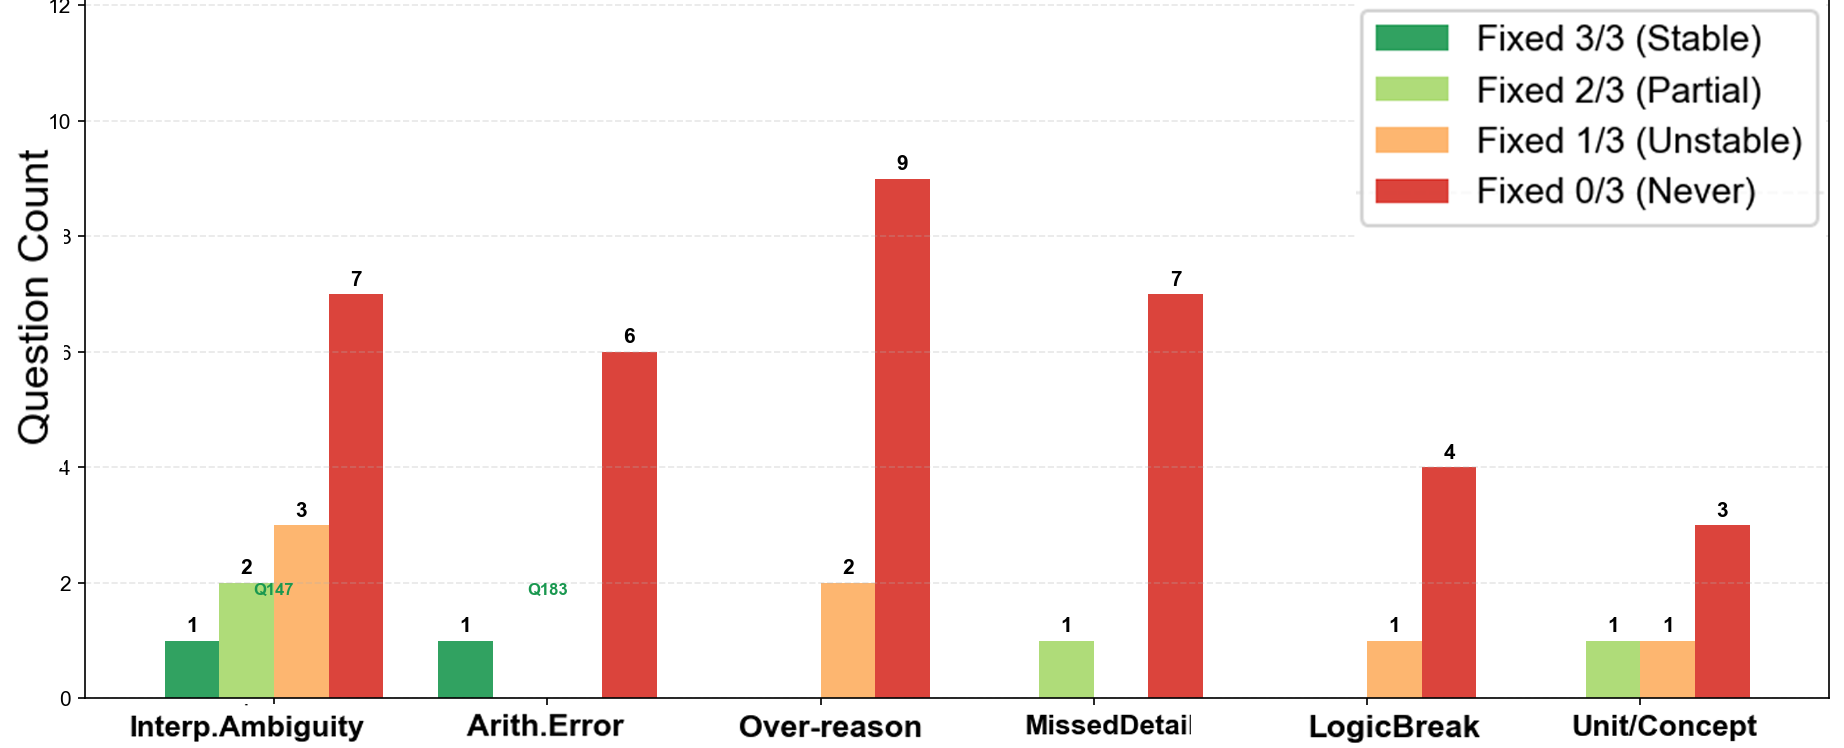
\includegraphics[width=\textwidth]{figures/fix_stability_by_cat.png}
    \caption{Fix stability distribution across 49 re-evaluated GSM8K problems over three prompt-augmented runs (RF2--RF4). Only 2 questions (4.1\%) are consistently fixed in all three rounds, while 40 (81.6\%) never recover. The high stochasticity undermines the reliability of single-run re-evaluations.}
    \label{fig:fix_stability_by_cat1}
\end{figure}
\begin{figure}[t]
    \centering
    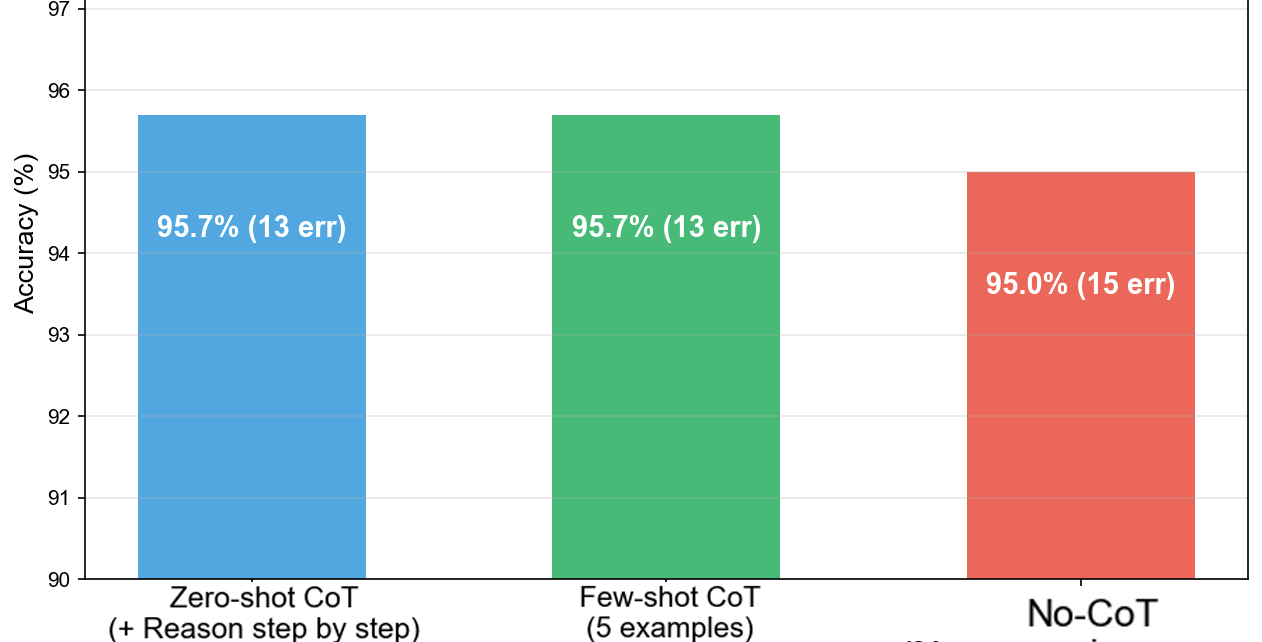
\includegraphics[width=0.8\columnwidth]{figures/three_prompt_accuracy_gsm8k.png}
    \caption{Accuracy of three prompting strategies on GSM8K Q1--300 (Qwen-Plus). Zero-shot CoT and Few-shot CoT achieve identical accuracy (95.7\%), while Direct Prompting trails marginally (95.0\%), indicating prompt saturation for strong models on simple tasks.}
    \label{fig:gsm300_accuracy1}
\end{figure}

Figure~\ref{fig:gsm300_accuracy1} presents the accuracy of the three strategies on GSM8K. See Section~\ref{sec:gsm300}.

\begin{figure*}[t]
    \centering
    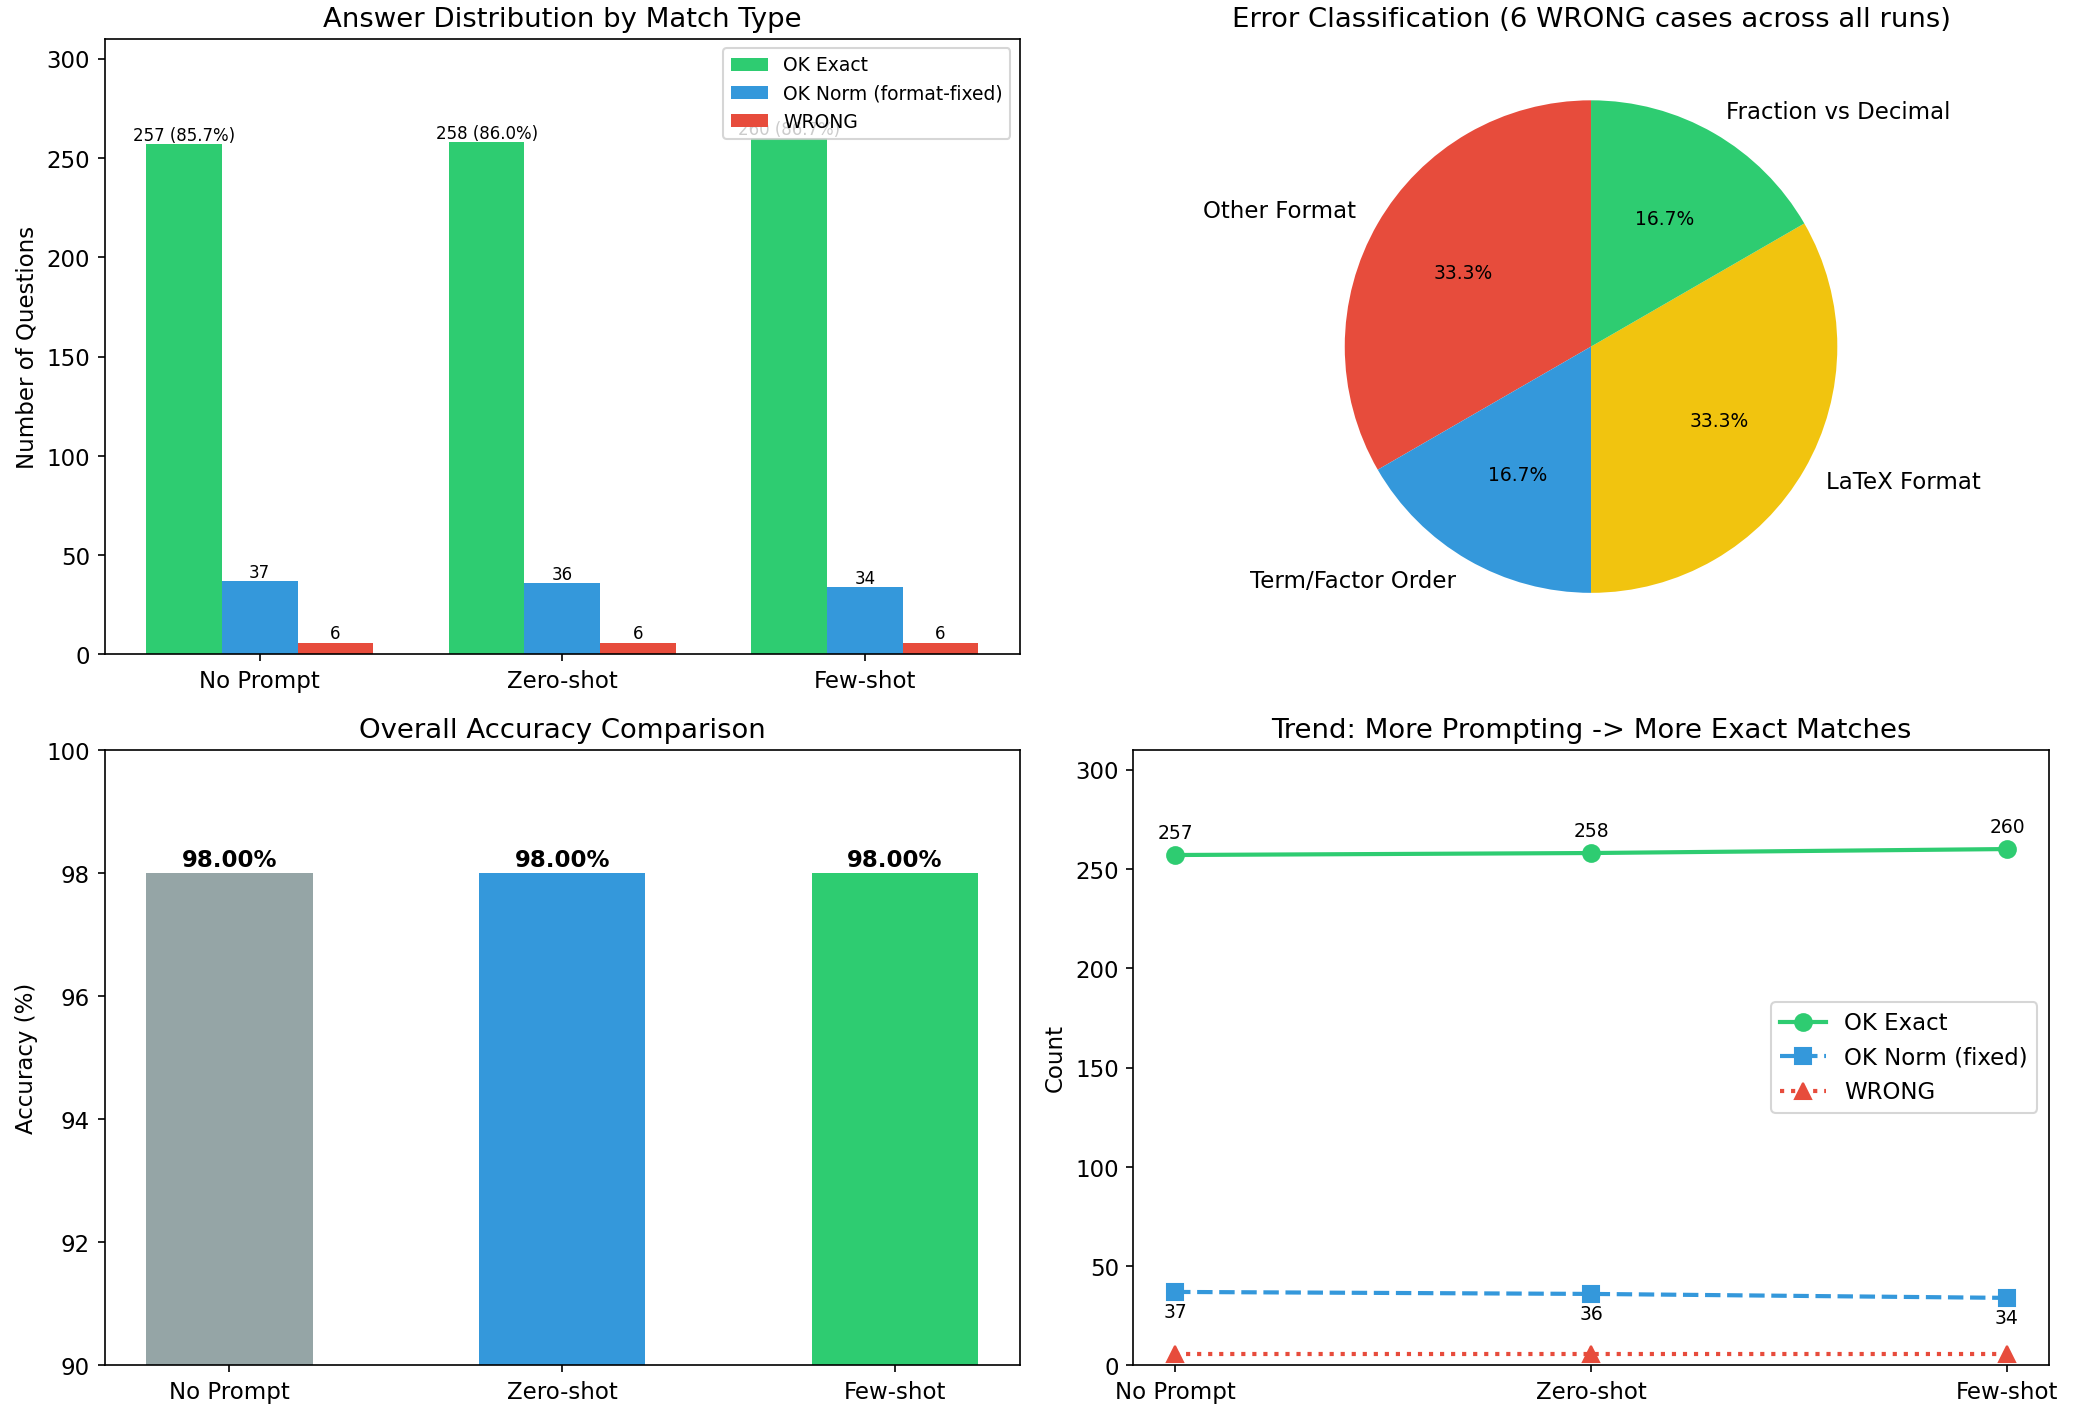
\includegraphics[width=\textwidth]{figures/plus_comparison_chart.png}
    \caption{MATH-Algebra (Q1--300) results for Qwen-Plus. Top-left: answer matching distribution. Top-right: error category breakdown (all format-related). Bottom-left: accuracy by strategy (all 98\%). Bottom-right: exact-match trend (257$\to$258$\to$260).}
    \label{fig:plus_math1}
\end{figure*}
Figure~\ref{fig:plus_math1} provide an overall analysis of the qwen-plus's performance using three prompt strategies. See Section~\ref{sec:math300}.
%----------------------------------------------------------------------

%----------------------------------------------------------------------
\section{Dataset-Level Annotation Errors}
\label{app:dataset_errors}
%----------------------------------------------------------------------

Figure~\ref{fig:annotation_errors} presents the complete details of the 7 problems in the GSM8K test set for which we identified inconsistencies between the problem statement and the reference solution. For each case, we independently recomputed the answer and confirmed that the model's output is mathematically correct. 
These cases are discussed in Section~\ref{sec:dataset_errors}.

\begin{figure}[h]
    \centering
    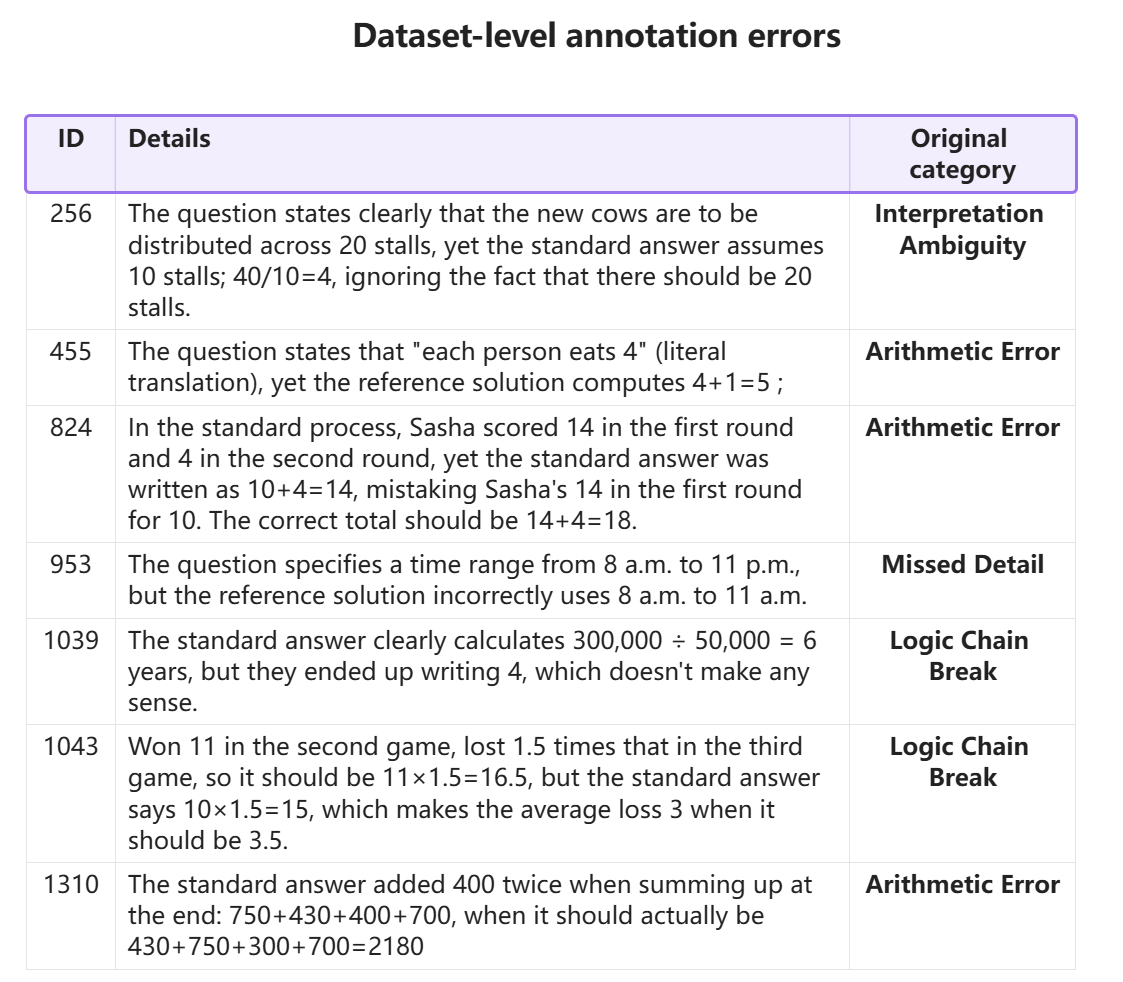
\includegraphics[width=\columnwidth]{figures/dataset_annotation_errors.png}
    \caption{Complete details of 7 dataset-level annotation errors identified in the GSM8K test set. For each problem, the table shows the problem ID, an abbreviated problem statement, the model's answer, the specific inconsistency in the reference solution, and the originally assigned error category. All 7 model outputs were verified to be mathematically correct.}
    \label{fig:annotation_errors}
\end{figure}


%----------------------------------------------------------------------
\section{Detailed Error Analysis}
\label{app:error_analysis}
%----------------------------------------------------------------------

\subsection{GSM8K Q1--300: Three-Strategy Error Comparison}
\label{app:gsm300_errors}

Figure~\ref{fig:gsm300_comparison} provides the per-question correctness comparison across all three prompting strategies on GSM8K Q1--300 (Qwen-Plus). This figure supports the analysis in Section~\ref{sec:gsm300}, including the identification of 6 shared failures and the zero-sum redistribution between Few-shot and Zero-shot CoT.

\begin{figure}[h]
    \centering
    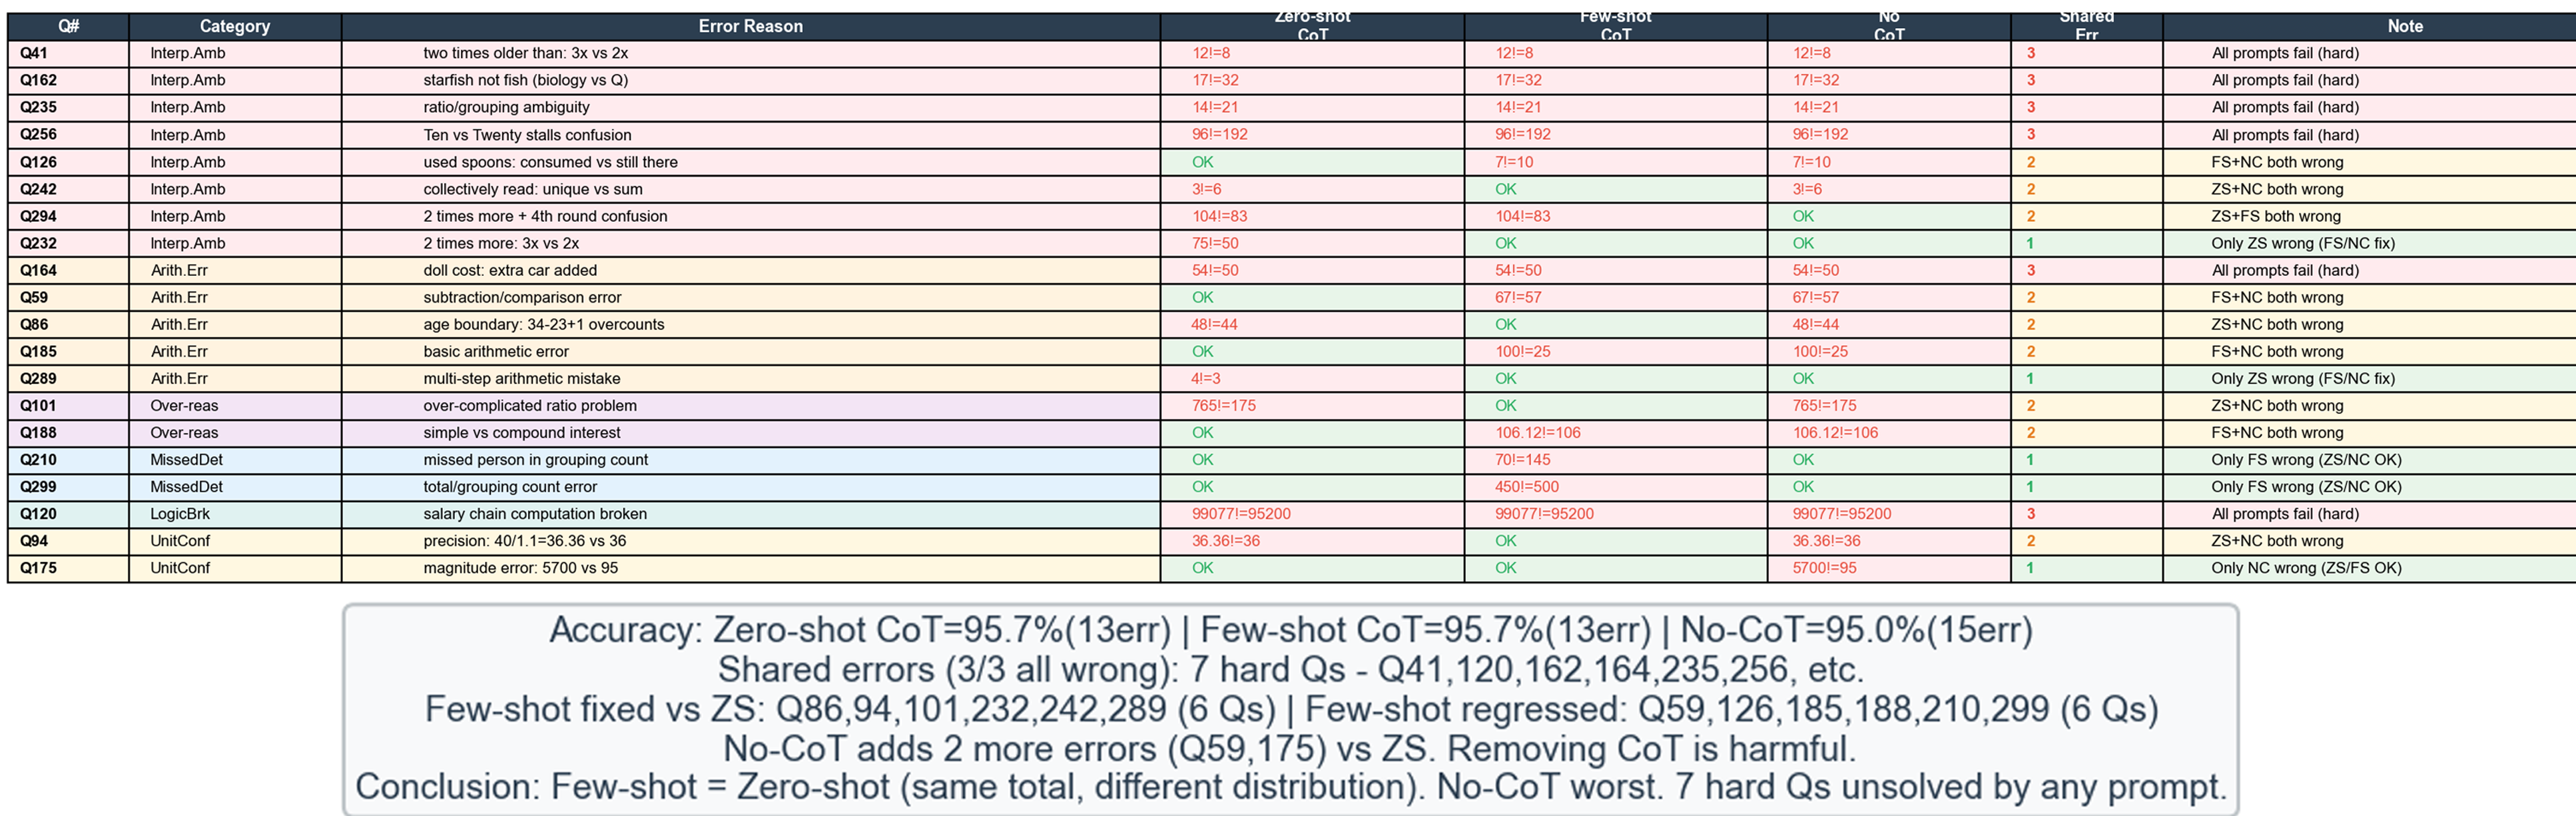
\includegraphics[width=\columnwidth]{figures/three_prompt_comparison1.png}
    \caption{Per-question correctness comparison across three prompting strategies (No-CoT, Zero-shot CoT, Few-shot CoT) on GSM8K Q1--300 (Qwen-Plus). A $\times$ indicates an incorrect answer. The 6 questions marked as shared failures are incorrectly answered under all three strategies. Few-shot CoT and Zero-shot CoT each have 13 errors but differ in which specific questions they miss, illustrating the zero-sum redistribution effect described in Section~\ref{sec:gsm300}.}
    \label{fig:gsm300_comparison}
\end{figure}


\subsection{Four-Round Iterative Re-evaluation: Per-Question Results}
\label{app:four_round}

Figure~\ref{fig:four_round_detail} reports the per-question outcomes across all four evaluation rounds (RF1--RF4) for the 49 initially incorrect GSM8K questions. This figure supports the stability analysis in Section~\ref{sec:stability}.

\begin{figure}[h]
    \centering
    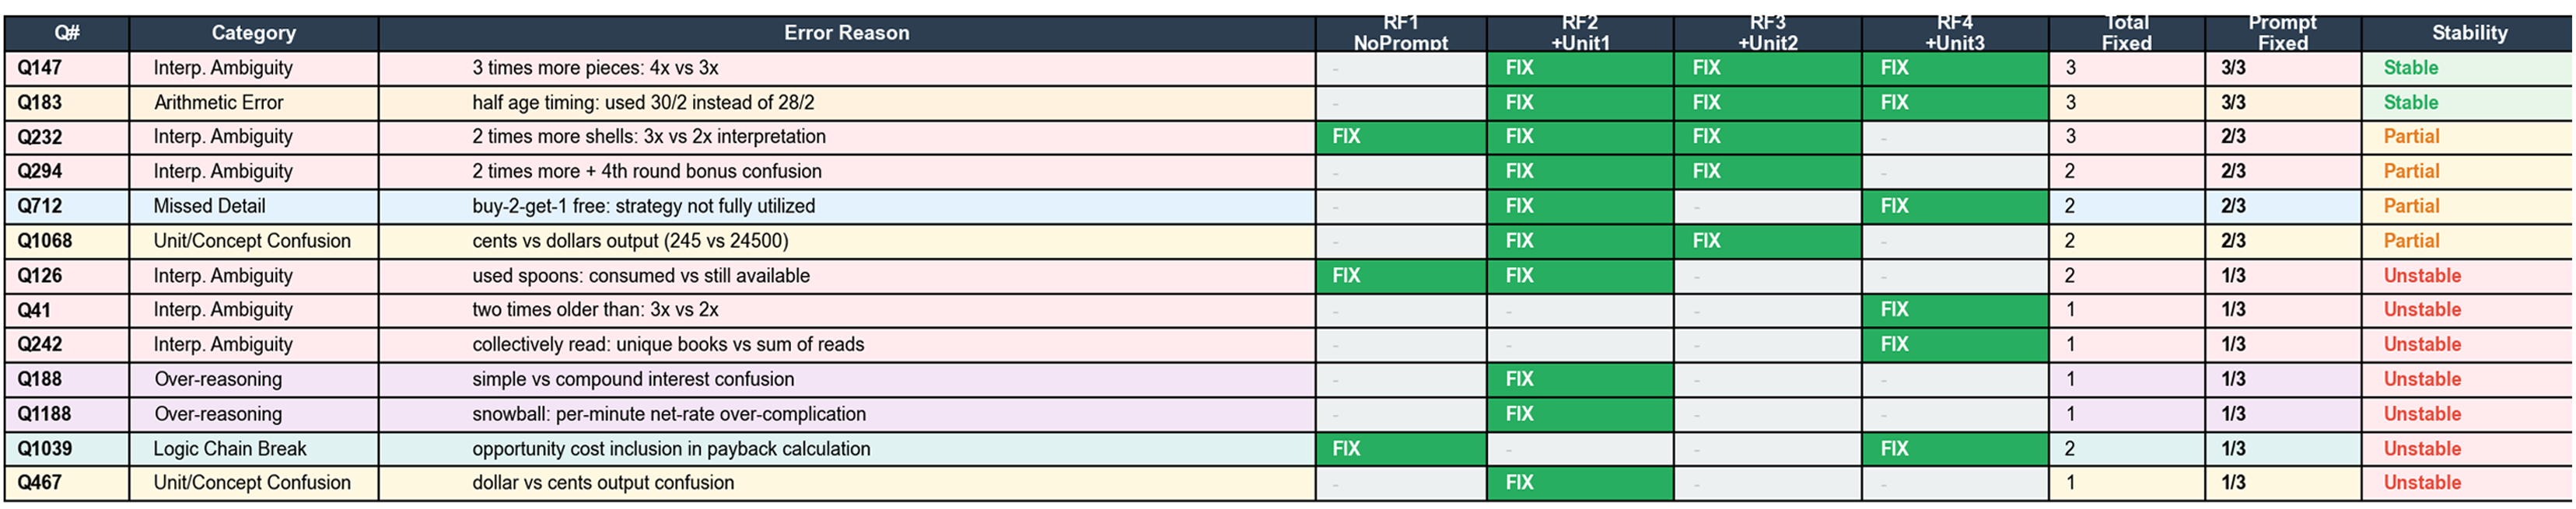
\includegraphics[width=\columnwidth]{figures/four_round_focused_table.png}
    \caption{Per-question recovery status across four evaluation rounds for the 49 initially incorrect GSM8K problems. RF1 uses the original Zero-shot CoT prompt; RF2--RF4 append a unit-conversion reminder. A $\checkmark$ indicates a correct answer in that round; $\times$ indicates an incorrect answer. The ``Fix Count'' column shows the number of prompt-augmented runs (RF2--RF4) in which the question was correctly answered. Only 2 questions (Q147, Q183) achieve a fix count of 3/3, while 40 questions never recover (0/3), confirming the high stochasticity reported in Section~\ref{sec:stability}.}
    \label{fig:four_round_detail}
\end{figure}


\subsection{MATH Turbo: Persistent Reasoning Errors}
\label{app:turbo_errors}

Figure~\ref{fig:turbo_persistent} extends the analysis in Section~\ref{sec:math300}(b) by listing all persistent reasoning errors of Qwen-Turbo on MATH-Algebra (Q1--300) across the three prompting strategies.

\begin{figure}[h]
    \centering
    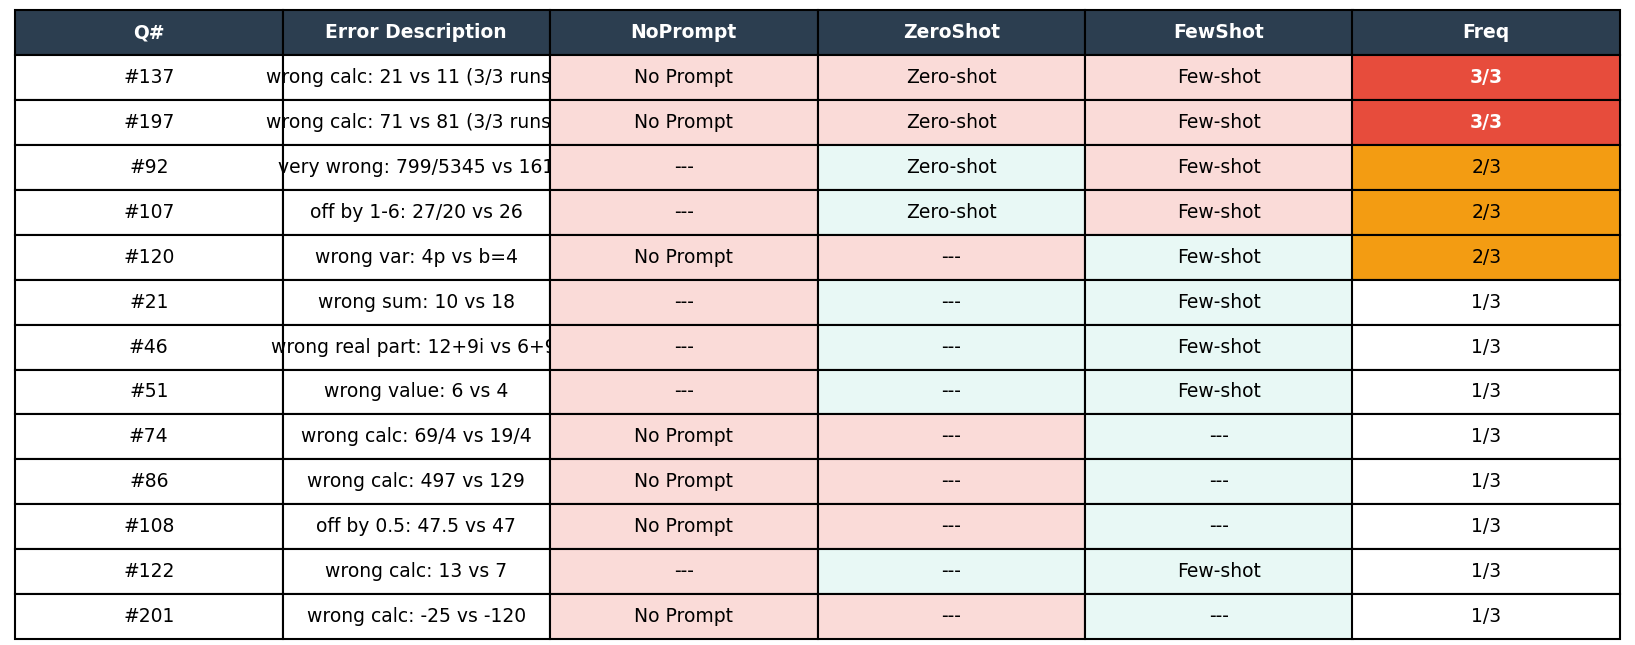
\includegraphics[width=\columnwidth]{figures/turbo_reasoning_errors_table.png}
    \caption{Persistent reasoning errors of Qwen-Turbo on MATH-Algebra (Q1--300) across three prompting strategies. A $-$ indicates an correct answer under that strategy. Problems \#137 and \#197 fail universally across all three configurations, indicating hard reasoning deficits. Problems \#21, \#46, \#51, and \#122 are uniquely missed by Few-shot CoT, providing direct evidence for the cognitive overload hypothesis discussed in Section~\ref{sec:math300}(b).}
    \label{fig:turbo_persistent}
\end{figure}


\end{document}